\documentclass{article}
\usepackage{amsmath}
\usepackage{amssymb}
\usepackage{graphicx}
\usepackage{hyperref}
\usepackage[version=4]{mhchem}

\title{Example 11}
\date{}

\begin{document}
\maketitle

\(A\) is a point outside the circle \(O\) of radius 1. \(O A=2 . A B\) is tangent to the circle at \(B\). Chord \(B C / / O A\). Connect \(A C\). Find the shaded area.

Solution: \(\frac{\pi}{6}\).\\
\centering
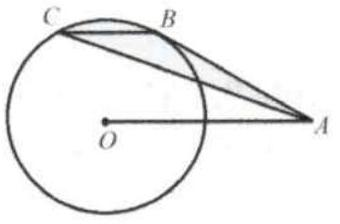
\includegraphics[width=\textwidth]{images/problem_image_1.jpg}

Connect \(O B, O C\). Since \(B C / / O A, S_{\triangle O B C}=S_{\triangle A B C}\).\\
Thus the shaded area is the same as the area of the sector \(O B C\).\\
Since \(A B\) is tangent to the circle, \(O B \perp A B\).\\
\centering
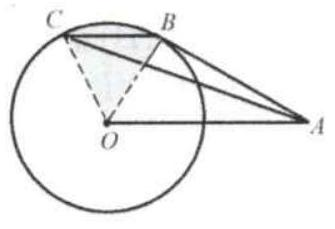
\includegraphics[width=\textwidth]{images/reasoning_image_1.jpg}

In right triangle \(A O B, A O=2, O B=1\). So \(\angle A O B=60^{\circ}\). So \(\angle B O C=60^{\circ}\).


The shaded area \(=\) the area of the sector \(\mathrm{OBC}=\pi \times \frac{1}{6}=\frac{\pi}{6}\).\\

\end{document}
